\documentclass[../TDT4.tex]{subfiles}%

\begin{document}
\section[s]"1"{Méthode des mélanges dans un calorimètre}
\enonce{%
	Un calorimètre de capacité thermique $C = \SI{150}{J.K^{-1}}$ contient
	initialement une masse $m_1 = \SI{200}{g}$ d'eau à $\theta_1 =
		\SI{20}{\degreeCelsius}$, en équilibre thermique avec le calorimètre. On plonge
	dans l'eau un bloc de fer de masse $m_2 = \SI{100}{g}$ initialement à la
	température $\theta_2 = \SI{80.0}{\degreeCelsius}$.
	\begin{tcn}(defi)<lftt>{Données}
		$c_{\ce{Fe}} = \SI{452}{J.K^{-1}.kg^{-1}}$ et $c_{\rm eau} =
			\SI{4185}{J.K^{-1}.kg^{-1}}$.
	\end{tcn}
}%

\QR{%
	Calculer la température d'équilibre $T_f$.
}{%
	Système = \{eau + calorimètre + fer\}~:
	\begin{center}
		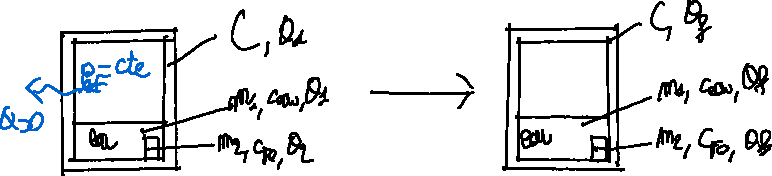
\includegraphics[scale=1]{E1_calo}
	\end{center}
	\begin{align*}
		\beforetext{Transformation isobare $\Ra$}
		\Delta{H} & = Q
		\\\beforetext{Calorifugé $Q = 0 \Ra$}
		\Delta{H} & = 0
		\\\beforetext{$H$ additive $\Ra$}
		m_1c\ind{eau} (T_f - T_1) + C (T_f - T_1) + m_2c_{\ce{Fe}}(T_f - T_2)
		          & = 0
		\\\Lra
		T_f \left( m_1c\ind{eau} + C + m_2c_{\ce{Fe}} \right)
		          & =
		T_1 \left( m_1c\ind{eau} + C \right) + T_2m_2c_{\ce{Fe}}
		\\\Lra
		\Aboxed{
		T_f       & =
		\frac{\left( m_1c\ind{eau} + C \right)T_1 + m_2c_{\ce{Fe}}T_2}
		{m_1c\ind{eau} + C + m_2c_{\ce{Fe}}}
		}
		\\
		\makebox[0pt][l]{$\phantom{\AN}\xul{\phantom{T_f = \SI{296}{K}}}$}
		\AN
		T_f       & = \SI{296}{K}
	\end{align*}
}%
\QR{%
	Calculer la variation d'entropie de l'eau, du fer et du calorimètre.
}{%
	Pour les phases condensées, $\DS \Delta{S} = C \ln \frac{T_f}{T_i}$~:
	\begin{align*}
		\Delta{S}\ind{eau}  & =
		m\ind{eau}c\ind{eau} \ln \frac{T_f}{T_1} = \xul{\SI{7.47}{J.K^{-1}}}
		\\
		\Delta{S}\ind{calo} & =
		C \ln \frac{T_f}{T_1} = \xul{\SI{1.34}{J.K^{-1}}}
		\\
		\Delta{S}\ind{fer}  & =
		m_2 c\ind{Fe} \ln \frac{T_f}{T_2} = \xul{\SI{-8.02}{J.K^{-1}}}
	\end{align*}
	\begin{tcn}(impo){Variation d'entropie}
		Attention, on n'a $\Delta{S} \geq 0$ \textbf{uniquement pour système isolé
			et à l'équilibre}~! On peut évidemment échanger de l'entropie entre les
		systèmes, donc l'un réduit d'entropie et l'autre augmente.
	\end{tcn}
}%
\QR{%
	En déduire l'entropie créée au cours de la transformation. Celle-ci
	est-elle réversible, et pourquoi~?
}{%
	Pour l'\textbf{ensemble}, $Q = 0$ donc $S\ind{ech,tot} = 0$. Ainsi,
	\[
		\boxed{S\ind{cr,tot} = \Delta{S}\ind{tot}}
		\Lra
		\xul{S\ind{cr,tot} = \SI{7.90e-1}{J.K^{-1}}} > 0
	\]
	On a donc une \textbf{transformation irréversible} à cause des
	\textbf{inhomogénéité de température}.
}%
\end{document}
